\documentclass[conference]{IEEEtran}
\IEEEoverridecommandlockouts
\usepackage{cite}
\usepackage{amsmath,amssymb,amsfonts}
\usepackage{graphicx}
\usepackage{textcomp}
\usepackage{booktabs}
\usepackage{url}

\begin{document}

\title{On-Device Acoustic Gunshot Detection: Data Cleaning, Model Comparison, and a One-Bit Edge Alert}

\author{
\IEEEauthorblockN{Jeevant Sharma, Deepesh Dangi, Abhishek Yadav, Bhupendra Kumar}
\IEEEauthorblockA{Department of Computer Science and Engineering\\
Indian Institute of Information Technology, Surat\\
Surat, India}
}

\maketitle

\begin{abstract}
A gunshot is a short impulse in a long recording, and the same shape appears in fireworks, hand claps, and door slams. This paper reports a detector aimed at an Arduino Nano 33 BLE Sense. Training and the tests here were done on a PC. Timing was measured on a virtual machine capped near 45--50\% CPU as a stand-in for a Raspberry Pi~4. No board has been flashed. Audio was cleaned with librosa at 250\,ms, 500\,ms, and 1\,s; the working window is 750\,ms because a 250\,ms cut drops the decay that separates a shot from a knock. Logistic regression, an SVM, and a random forest reached about 99--100\% on some balanced files and failed on a live microphone. On a 1{,}442-clip balanced hold-out, three neural models exceed 99.5\% accuracy. On 300 unseen recordings the best sliding-window gunshot recall is 67\%. The Enhanced 2D CNN runs in 0.09\,ms inside 123.6\,KB (INT8). The deployment design keeps audio on the node, sleeps between loud frames, and transmits a single bit: 1 if the score crosses the threshold, and nothing otherwise. A gateway accepts an event only when several nearby nodes send that bit. The bit is a binary decision from an ordinary network, not a weight-binarized neural network.
\end{abstract}

\begin{IEEEkeywords}
Acoustic gunshot detection, edge inference, TinyML, PCEN, Raspberry Pi, Arduino Nano 33 BLE Sense.
\end{IEEEkeywords}

\section{Introduction}
\label{sec:intro}
In some countries a person may carry a firearm with a licence. Elsewhere the same sound on a street is a crime. People nearby do not always call, and a call that does arrive is often late and poorly located. A campus, a city block, or a forest sanctuary can listen for the sound and send medical help and police to the place of the event. The same listening problem appears where a gunshot or a chainsaw is rare against hours of wind. We did not build a chainsaw detector. We reuse a front-end that was developed for that kind of rare impulse.

A dense city is a hard first site. Traffic and fireworks produce impulses all day. A college or a school is a smaller site with a known map, which is where we intend to start.

The final node is an Arduino Nano 33 BLE Sense. It should run the model locally and should not stream the microphone. This paper stops one step earlier. Models were trained on a PC, converted from Keras to TensorFlow Lite, and timed on a virtual Raspberry Pi. The value that leaves the node is a binary label. Sleep, the radio, and gateway grouping are the next build. They were not measured here.

Section~\ref{sec:related} is related work. Section~\ref{sec:method} is the method. Section~\ref{sec:setup} defines the tests and the metrics. Section~\ref{sec:results} gives the numbers. Section~\ref{sec:conclusion} states what failed and what the hardware step is.

\section{Related Work}
\label{sec:related}
Acoustic gunshot detection already exists as a city product and as a public dataset. We use firearm recordings that include the multi-firearm, multi-orientation set in \emph{Data in Brief}~\cite{dib2023}. Those systems also show the constraint we care about: a campus node should not upload the microphone.

Per-channel energy normalization (PCEN) divides each frequency band by a running estimate of its own background, so steady rain and hum flatten and a short impulse does not~\cite{lostanlen2019}. One of our models uses that front-end. The data, the network, and the tests are ours. Forest monitors that listen for chainsaws are a separate existing service. We did not reimplement them.

Edge Impulse was a separate TinyML trial on a Cortex-M4F class target. It is a tool we used, not an architecture we claim. Mixup~\cite{zhang2018} and SpecAugment~\cite{park2019} appear only as regularization inside the enhanced convolutional models. Spatial grouping in Section~\ref{sec:conclusion} is a count of nearby detection bits inside a short time window.

\section{Method}
\label{sec:method}

\subsection{Cleaning and window length}
The raw pool was on the order of 80{,}000 files from firearm sets and long ambient recordings. Cleaning used librosa. About 1{,}000 to 5{,}000 clips were listened through in cycles until the remaining cuts were acceptable.

Cuts were made at 250\,ms, 500\,ms, and 1\,s. The muzzle attack lasts only a few milliseconds. The decay that follows often lasts a few hundred milliseconds. A 250\,ms cut keeps the attack and drops most of that decay, so a shot and a knock become similar. The neural models use \textbf{750\,ms} (16{,}537 samples at 22{,}050\,Hz). On the live path, windows overlap by 75\% (hop 187.5\,ms) so a blast on a boundary still falls inside one frame.

Negative clips that were themselves sharp knocks were removed when crest factor and attack energy matched a shot. The negative class has to be ordinary sound.

A 1:1 training folder is easy to score and is what produced the classical 99--100\% figures. Continuous monitoring is closer to 1:10 or 1:50, because almost every window is silence, speech, or traffic. Later training used a larger negative set. A model shown only a coin-flip folder calls too many ordinary sounds a shot.

\subsection{Classical models}
Logistic regression was a probe: could a threshold on hand-made features separate the classes at all? It is a weak final model here. The classes are not a straight line in MFCC space, and a live threshold has to survive sounds the folder never held. An SVM and a random forest were then trained on MFCC and related summaries, from a 1:1 balance toward 1:10.

On held-out files from the same pool, some of these runs sat near 99--100\% accuracy. On a real microphone they did not. Averaging a clip into a few MFCCs erases the few-millisecond attack. Keys, brakes, and claps land in a similar summary. The classical classifiers stopped there.

\subsection{Edge Impulse trial}
Five Edge Impulse configurations were run before the TensorFlow models. Validation accuracy was high. Live audio was not. MFCC with a 1D CNN marked 33 of 47 speech and ambient windows as shots. A 2D CNN on a mel spectrogram was the first run that rejected heavy wind on about 76\% of windows and thunder on about 80\%, at 99.6\% validation accuracy, 167\,ms INT8 inference, 30.2\,KB RAM, and 52.2\,KB flash on the M4F target. That latency is uncomfortable on a 64\,MHz part. The trial is why we moved to our own spectrogram CNNs. It is not the system we would ship.

\subsection{Neural models}
Five models share the 750\,ms front-end. The device path subtracts the sample mean so a small microphone DC bias is not treated as energy. Peak scaling runs only when the window RMS is high enough. Scaling a near-silent window up to full scale turns ADC hiss into a loud signal.

\begin{table}[!t]
\centering
\caption{Models scored in this paper.}
\label{tab:models}
\footnotesize
\begin{tabular}{lrr}
\toprule
\textbf{Model} & \textbf{Parameters} & \textbf{INT8} \\
\midrule
Baseline 1D CNN (waveform) & 92{,}513 & 112.5\,KB \\
Baseline 2D CNN (log-mel) & 249{,}985 & 259.9\,KB \\
Enhanced 1D CNN & 96{,}674 & 118.5\,KB \\
Enhanced 2D CNN (log-mel) & 110{,}594 & 123.6\,KB \\
CRNN-PCEN + Bi-GRU & 397{,}842 & 478.9\,KB \\
\bottomrule
\end{tabular}
\end{table}

The 1D network uses a first kernel of 80 samples (about 3.6\,ms), wide enough to see a short attack. An early 2D run fed decibel values from about $-80$\,dB to $0$\,dB into ReLU. ReLU outputs zero on the whole range, training stalled, and that checkpoint scored all 721 hold-out gunshots as negatives. Later 2D models use $(S_{\mathrm{dB}}+80)/80$, which maps the image into $[0,1]$.

The enhanced models add mixup and, on the 2D path, SpecAugment, plus a second head used as an anomaly score. The enhanced 1D model was trained with a heavy penalty on missed shots. After INT8 conversion it scores every window as a gunshot. We report it as a failed conversion.

PCEN replaces the static log-mel in the CRNN. A smoothed background $M[f,t]$ tracks each mel band $S[f,t]$:
\begin{equation}
P[f,t] = \left( \frac{S[f,t]}{(\epsilon + M[f,t])^{\alpha}} + \delta \right)^{r} - \delta^{r}.
\label{eq:pcen}
\end{equation}
With $\alpha$ near 0.98, a band that stays constant collapses toward 1. A short blast does not. PCEN needs a real impulse-plus-background recording. A bad trim leaves nothing stable to track, which is why cleaning comes first.

Figure~\ref{fig:pipeline} is the path from the microphone to the bit. Audio stays on the node.

\begin{figure}[!t]
\centering
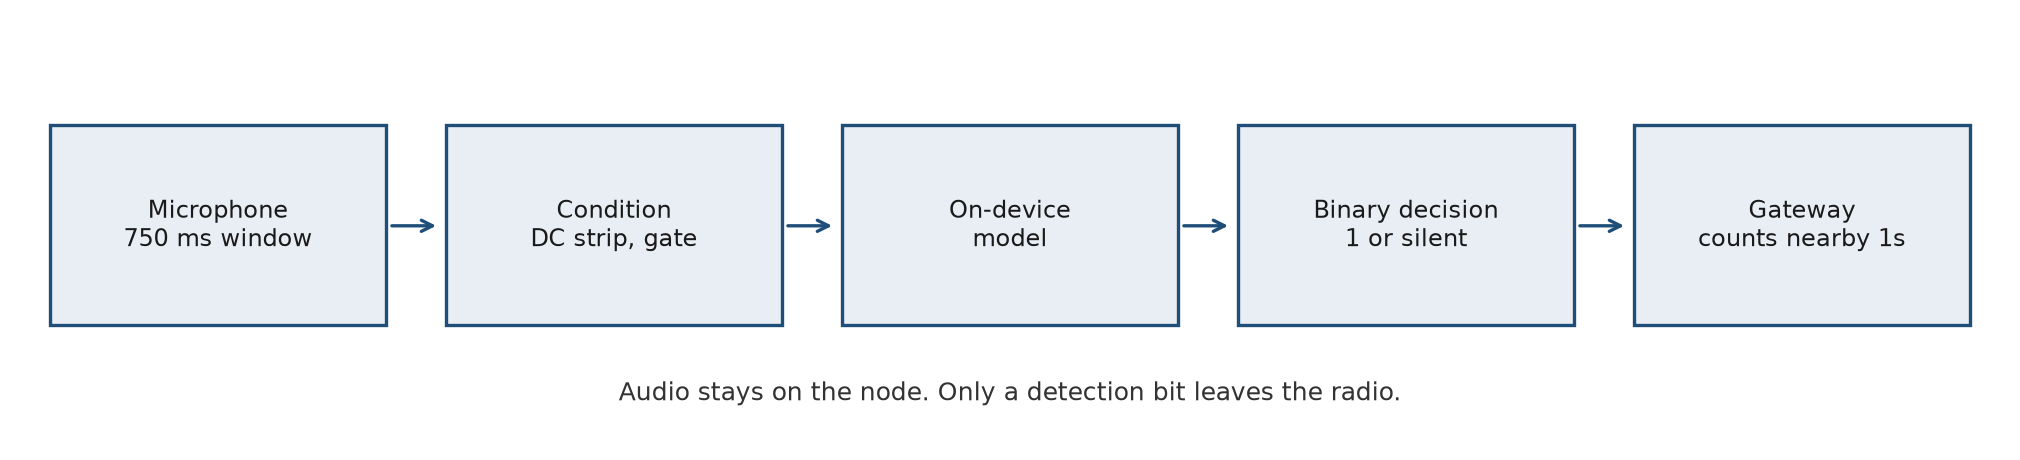
\includegraphics[width=\columnwidth]{figures/fig1_edge_pipeline.png}
\caption{Node path. The gateway sees detection bits, not audio.}
\label{fig:pipeline}
\end{figure}

\section{Setup and Metrics}
\label{sec:setup}
Neural scores were computed in software. Latency is from a virtual Raspberry Pi~4 (four virtual CPUs, execution cap about 45--50\%, 2\,GB RAM), 100 iterations per model. A balanced hold-out has 1{,}442 clips of 750\,ms (721 gunshot, 721 other). An earlier external check has 75 recordings (20 firearms, 20 imposters, 35 ambient). The main unseen set has 300 recordings with no training overlap: 100 real gunshots, 100 ambient files, and 100 hard imposters.

Accuracy on a 1:1 folder is reported because that is what a balanced test produces. It is not how we choose a model. A detector that always says ``not a gunshot'' can look accurate whenever most audio is background.

Gunshot recall is the fraction of real gunshot files that cross the threshold. Ambient specificity is the fraction of rain, traffic, and speech files that stay below it. Imposter rejection is the fraction of fireworks, claps, and other bangs that stay below it. Latency is the time to score one window. The live hop is 187.5\,ms. INT8 size is listed because the Nano 33 BLE Sense has a small flash budget. The threshold is 0.50 unless a row says otherwise.

Peak-centered scoring uses one 750\,ms slice around the loudest sample. Sliding scoring walks the window across the file. Sliding finds more shots and more false alarms.

\section{Results}
\label{sec:results}

\subsection{Balanced hold-out}
Table~\ref{tab:holdout} is the near-100\% 1:1 result. It checks that training ran.

\begin{table}[!t]
\centering
\caption{Hold-out, 1{,}442 clips, threshold 0.50.}
\label{tab:holdout}
\footnotesize
\begin{tabular}{lccc}
\toprule
\textbf{Model} & \textbf{Acc.} & \textbf{Recall} & \textbf{FP} \\
\midrule
Baseline 1D CNN & 99.79\% & 99.72\% & 1 \\
CRNN-PCEN & 99.79\% & 99.72\% & 1 \\
Enhanced 2D CNN & 99.51\% & 99.58\% & 4 \\
2D CNN, unscaled dB & 50\% & 0\% & 0 \\
Enhanced 1D CNN & 50\% & 100\% & 721 \\
\bottomrule
\end{tabular}
\end{table}

The unscaled 2D row is the stalled checkpoint (721 false negatives). The 2D model in Table~\ref{tab:slide} is a later checkpoint. The enhanced 1D row is positive on every file.

\subsection{Seventy-five external recordings}
A file counts as a detection if any 750\,ms window at 75\% overlap crosses 0.50. Enhanced 2D recall is 17/20 shots with 33/35 ambient files ignored and 7/20 imposters rejected. CRNN-PCEN recall is 12/20 with all 35 ambient files ignored and 8/20 imposters rejected. Baseline 1D recall is 6/20. Figure~\ref{fig:drop} places this next to the hold-out. The 1D model has memorized training waveforms. On one 35-window clapping file, PCEN fired on 23 windows: it boosts any fast transient.

\begin{figure}[!t]
\centering
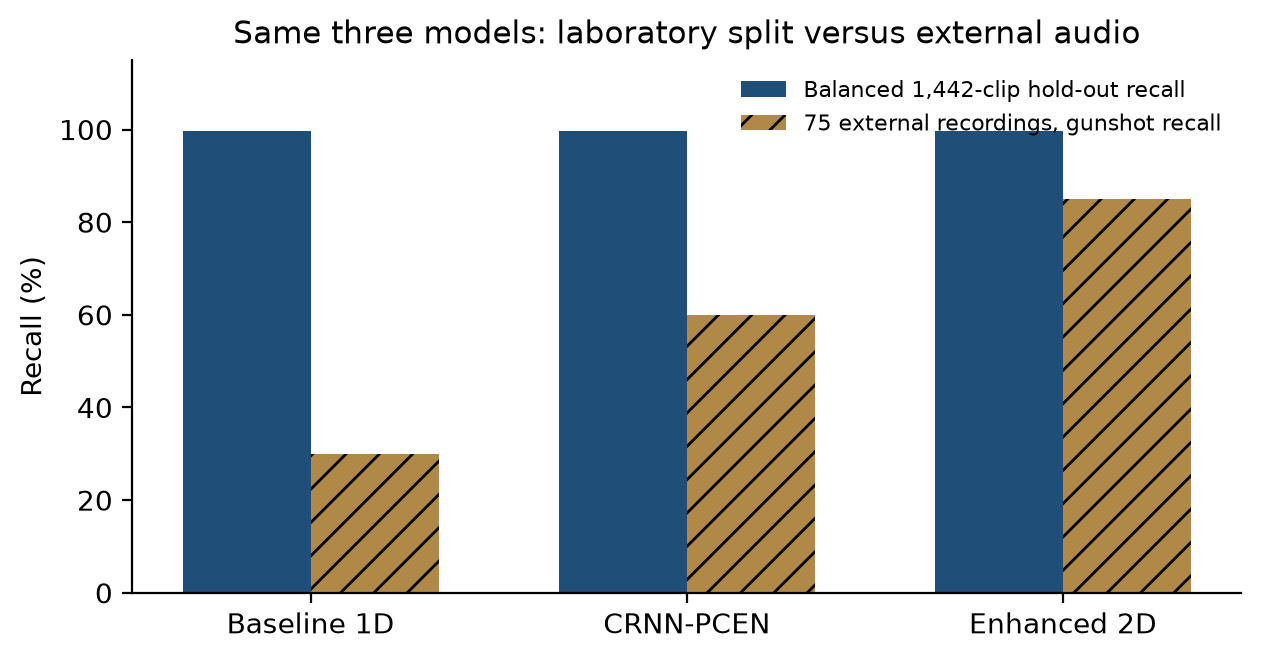
\includegraphics[width=\columnwidth]{figures/fig4_lab_vs_external.png}
\caption{Hold-out recall versus recall on 75 external recordings.}
\label{fig:drop}
\end{figure}

\subsection{Three hundred unseen clips}
Tables~\ref{tab:slide} and~\ref{tab:peak} are the main result (INT8, threshold 0.50, virtual Raspberry Pi).

\begin{table}[!t]
\centering
\caption{Sliding window, 300 clips.}
\label{tab:slide}
\footnotesize
\begin{tabular}{lccc}
\toprule
\textbf{Model} & \textbf{Recall} & \textbf{Ambient} & \textbf{Imposter} \\
\midrule
Baseline 1D & 45\% & 85\% & 72\% \\
Baseline 2D & 66\% & 88\% & 59\% \\
Enh. 1D (broken) & 100\% & 0\% & 0\% \\
Enhanced 2D & 67\% & 82\% & 66\% \\
CRNN-PCEN & 57\% & 86\% & 61\% \\
\bottomrule
\end{tabular}
\end{table}

\begin{table}[!t]
\centering
\caption{Peak-centered window, 300 clips.}
\label{tab:peak}
\footnotesize
\begin{tabular}{lccc}
\toprule
\textbf{Model} & \textbf{Recall} & \textbf{Ambient} & \textbf{Imposter} \\
\midrule
Baseline 1D & 30\% & 95\% & 84\% \\
Baseline 2D & 45\% & 94\% & 77\% \\
Enh. 1D (broken) & 100\% & 0\% & 0\% \\
Enhanced 2D & 38\% & 99\% & 89\% \\
CRNN-PCEN & 33\% & 97\% & 85\% \\
\bottomrule
\end{tabular}
\end{table}

\begin{figure}[!t]
\centering
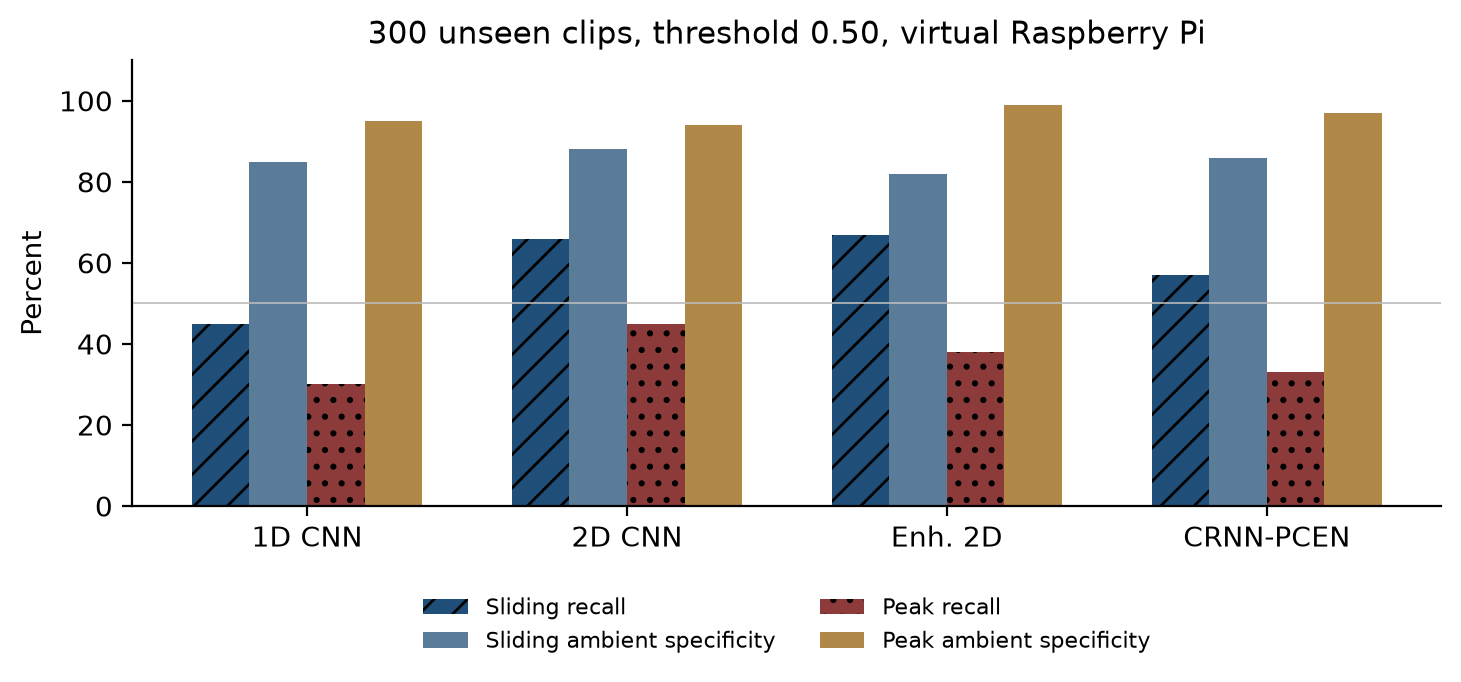
\includegraphics[width=\columnwidth]{figures/fig2_300clip_recall.png}
\caption{Working models on 300 clips. Sliding recall is higher. Peak specificity is higher.}
\label{fig:300}
\end{figure}

Sliding recall is 15 to 29 points above peak recall for every working model. A crop around the loudest sample misses shots whose energy is spread out. Host versus virtual-machine peak recall differs by about 4 to 6 points (enhanced 2D: 44.1\% host, 38.0\% VM; CRNN-PCEN: 32.0\% and 33.0\%). Model order does not change.

\subsection{Latency}
Table~\ref{tab:latency} and Fig.~\ref{fig:lat} use 100 iterations. Every model finishes inside the 187.5\,ms hop on this virtual machine. The enhanced 2D CNN is the small file with the best sliding recall among models that still discriminate. The CRNN is the model whose recall moves least under a distorted microphone, at a larger file.

\begin{table}[!t]
\centering
\caption{INT8 latency on the capped virtual machine.}
\label{tab:latency}
\footnotesize
\begin{tabular}{lcc}
\toprule
\textbf{Model} & \textbf{Mean} & \textbf{Hop used} \\
\midrule
Baseline 1D CNN & 2.29\,ms & 1.2\% \\
Baseline 2D CNN & 2.15\,ms & 1.2\% \\
Enhanced 1D CNN & 2.69\,ms & 1.4\% \\
Enhanced 2D CNN & 0.09\,ms & 0.05\% \\
CRNN-PCEN & 11.86\,ms & 6.3\% \\
\bottomrule
\end{tabular}
\end{table}

\begin{figure}[!t]
\centering
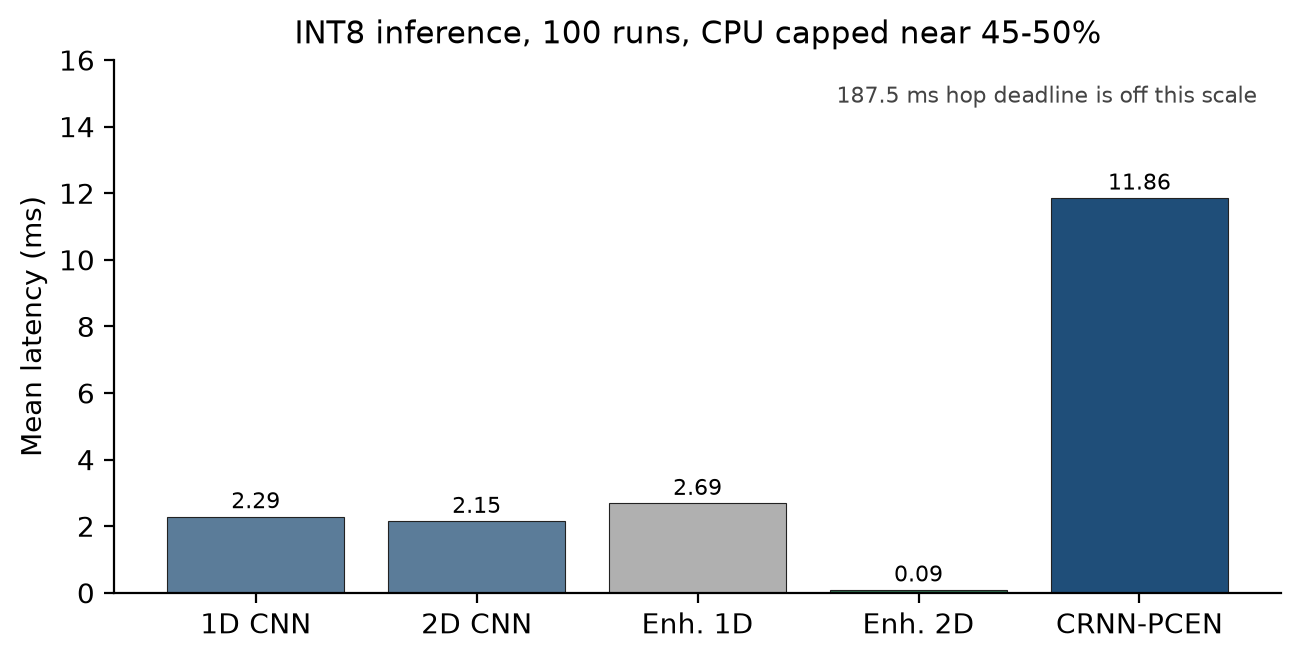
\includegraphics[width=\columnwidth]{figures/fig3_latency.png}
\caption{Mean INT8 latency. The 187.5\,ms hop is far above this range.}
\label{fig:lat}
\end{figure}

\subsection{PCEN and the ensemble}
The CRNN input was band-limited, clipped, gained, and noised. Sliding recall at threshold 0.50 was 61\% clean and 61\% distorted (69\% on both at threshold 0.10). A change of capsule does not by itself wipe recall. Fireworks and claps remain, because they are impulses too (Fig.~\ref{fig:pcen}).

\begin{figure}[!t]
\centering
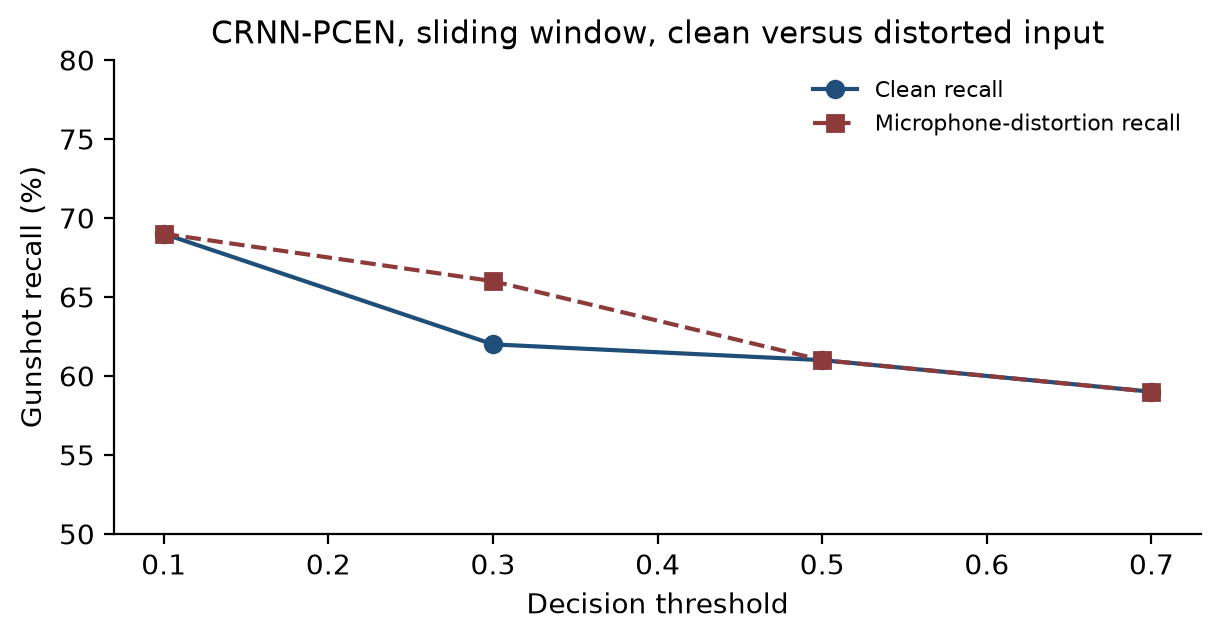
\includegraphics[width=\columnwidth]{figures/fig6_pcen_distortion.png}
\caption{CRNN-PCEN sliding recall, clean input versus simulated microphone distortion.}
\label{fig:pcen}
\end{figure}

An ensemble of the enhanced 2D CNN, the CRNN, and the baseline 1D CNN calls 77 of 100 real shots correctly (Fig.~\ref{fig:cm}). It also calls 44 of 100 imposters real shots, and 20 of 100 ambient files real shots. Combined size is about 715\,KB and combined time about 17\,ms. For a first campus node the single enhanced 2D model is the practical choice. The ensemble is the higher-recall option if the gateway can tolerate more false bits.

\begin{figure}[!t]
\centering
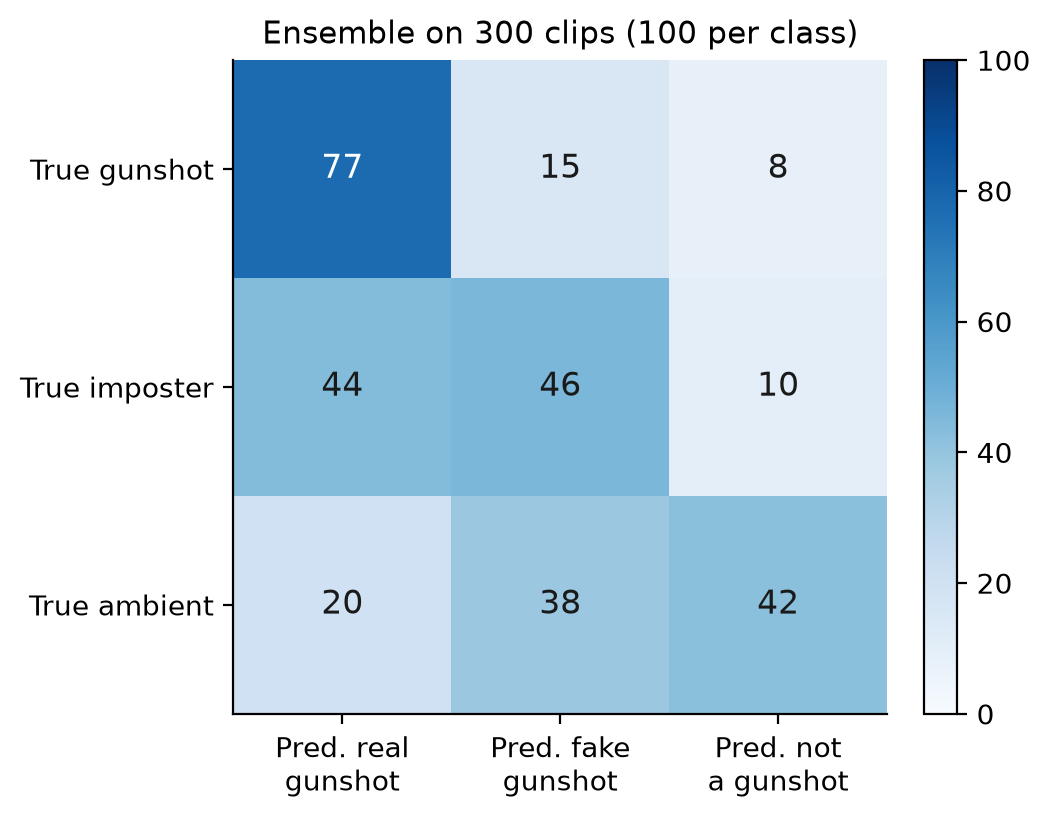
\includegraphics[width=\columnwidth]{figures/fig5_ensemble_confusion.png}
\caption{Ensemble counts on 300 clips, 100 files per true class.}
\label{fig:cm}
\end{figure}

The 99\% hold-out and the 99\% Edge Impulse scores are folder scores. The 300-clip test matches the original problem: most audio is not a shot, and many loud sounds are not shots either. No single model is both highly sensitive and highly specific. One microphone has no second arrival time with which to separate a firework from a shot.

\section{Conclusion}
\label{sec:conclusion}
We cleaned a large pool, dropped the 250\,ms cut, and showed that SVM and random-forest scores near 100\% on a balanced file test do not survive a live microphone. A 2D spectrogram CNN is the first model that rejects a useful share of wind, rain, and traffic. On 300 unseen clips the enhanced 2D CNN reaches 67\% gunshot recall when the window slides and 99\% ambient specificity on a peak crop, in 0.09\,ms and 124\,KB. The PCEN-CRNN stays stable when the microphone is distorted, at lower recall and a larger file. The enhanced 1D network is not usable after INT8 conversion.

These tests ran on a PC and on a virtual Raspberry Pi. The Arduino Nano 33 BLE Sense has not been programmed. The remaining work is hardware.

\emph{Sleep.} The node should stay idle until the sound level crosses a coarse threshold, run one inference, and return to idle. We have not measured that current.

\emph{One-bit transmission.} If the score crosses the threshold the node sends 1, with a node id and a timestamp. Otherwise the radio stays off. Raw audio is never sent. In our notes this was called a binary neural network. The accurate description is an ordinary network with a binary decision. Weights were not binarized. The energy saving comes from not sending audio, and from not sending anything on the zeros. It has not been metered.

\emph{Aggregation.} One node beside a clap will sometimes send a 1. The gateway should alarm only when more than one nearby node sends a 1 inside the short time sound takes to cross the site. That is a count and a time check. It is how a single microphone's false bit from a clap or a firework gets dropped. It is not built yet.

The next build is to put the enhanced 2D INT8 model on a physical Raspberry Pi, check the virtual-machine timing, and then move the same binary decision onto the Nano 33 BLE Sense.

\section*{Acknowledgment}
Firearm recordings include the open set of~\cite{dib2023}. PCEN follows~\cite{lostanlen2019}. The advisor for this project is Dr. Kaustubh Dhondge.

\begin{thebibliography}{4}
\bibitem{dib2023} ``A multi-firearm, multi-orientation audio dataset of gunshots,'' \emph{Data in Brief}, vol. 48, Art. no. 109091, 2023, doi: 10.1016/j.dib.2023.109091.
\bibitem{lostanlen2019} V. Lostanlen, J. Salamon, M. Cartwright, B. McFee, A. Farnsworth, S. Kelling, and J. P. Bello, ``Per-channel energy normalization: Why and how,'' \emph{IEEE Signal Process. Lett.}, vol. 26, no. 1, pp. 39--43, 2019.
\bibitem{zhang2018} H. Zhang, M. Cisse, Y. N. Dauphin, and D. Lopez-Paz, ``mixup: Beyond empirical risk minimization,'' in \emph{Proc. ICLR}, 2018.
\bibitem{park2019} D. S. Park \emph{et al.}, ``SpecAugment: A simple data augmentation method for automatic speech recognition,'' in \emph{Proc. Interspeech}, 2019, pp. 2613--2617.
\end{thebibliography}

\end{document}
